%% PROPOSAL: Generation of elliptic curves for circuit use.
%% Marta, Barry and Jordi.
%% The 2nd ZKProof Workshop 2019.

% TODO: Posar la bibliografia com toca (manera rara de referenciar).
% TODO: Larger space between text and page number.
% TODO: Zcash has been pioneer in all this framework. This is the result of 2nd ZKProof Workshop which took place ... .

\documentclass{article}
\setlength{\columnsep}{0.8cm} %Space between columns

% Packages
	\usepackage[colorlinks=true,
				urlcolor=black,
				linkcolor=black,
				citecolor=black
				]{hyperref} 
	
	\usepackage[english]{babel}
	\usepackage[utf8]{inputenc}
	\usepackage{amsmath, amsthm, amssymb, mathtools}
	\usepackage{enumerate, enumitem}
	\usepackage{graphicx, color, xcolor}
	\usepackage{setspace}
	\usepackage{authblk}
	\usepackage{braket}
	
	\usepackage{multicol, multirow}
	\usepackage{makecell} %Per fer línies en negreta
	\usepackage{array}
	\newcolumntype{?}{!{\vrule width 1pt}}
	
	\usepackage[linesnumbered,ruled,vlined]{algorithm2e}
		
	\usepackage{listings}
	\lstdefinelanguage{Sage}[]{Python}
	{morekeywords={False,sage,True},sensitive=true}
	\lstset{frame=none,
			showtabs=False,
			showspaces=False,
			showstringspaces=False,
			commentstyle={\ttfamily\color{dgreencolor}},
			keywordstyle={\ttfamily\color{dbluecolor}\bfseries},
			stringstyle={\ttfamily\color{dgraycolor}\bfseries},
			language=Sage,
			basicstyle={\fontsize{10pt}{10pt}\ttfamily},
			aboveskip=0.3em,
			belowskip=0.1em,
			numbers=none,%left,
			numberstyle=\footnotesize
			}
		
	\definecolor{dblackcolor}{rgb}{0.0,0.0,0.0}
	\definecolor{dbluecolor}{rgb}{0.01,0.02,0.7}
	\definecolor{dgreencolor}{rgb}{0.2,0.4,0.0}
	\definecolor{dgraycolor}{rgb}{0.30,0.3,0.30}
	\newcommand{\dblue}{\color{dbluecolor}\bf}
	\newcommand{\dred}{\color{dredcolor}\bf}
	\newcommand{\dblack}{\color{dblackcolor}\bf}

% Commands	
	\newcommand{\N}{\ensuremath{\mathbb{N}}}
	\newcommand{\Np}{\ensuremath{\mathbb{N}^{+}}}
	\newcommand{\Z}{\ensuremath{\mathbb{Z}}}
	\newcommand{\Q}{\ensuremath{\mathbb{Q}}}
	\newcommand{\R}{\ensuremath{\mathbb{R}}}
	\newcommand{\C}{\ensuremath{\mathbb{C}}}
	\newcommand{\Fp}{\ensuremath{\mathbb{F}_p}}
	\newcommand{\Fr}{\ensuremath{\mathbb{F}_r}}
	\newcommand{\G}{\ensuremath{\mathbb{G}}}
	\newcommand{\point}[1]{P_{#1} = (x_{#1}, y_{#1})}
	\newcommand{\llog}{\log_2}
	\newcommand{\xor}{\oplus}
	\newcommand{\minSize}{1.5em}
	\newcommand{\gen}[1]{\ensuremath{\langle #1\rangle}}
	\newcommand{\noi}{\noindent}
	\newcommand{\red}[1]{\textcolor{red}{#1}}
	\newcommand{\blue}[1]{\textcolor{blue}{#1}}

% Theorems and stuff
	%\theoremstyle{plain}  
	\newtheorem{thm}{Theorem}[section]
	\newtheorem{lem}[thm]{Lemma}
	\newtheorem{prop}[thm]{Proposition}
	\newtheorem{cor}[thm]{Corollary}
	\newtheorem{grouplaw}[thm]{Group Law}
	\newtheorem{prob}[thm]{Problem}
	\theoremstyle{definition}
	\newtheorem{defn}[thm]{Definition}
	\theoremstyle{remark}
	\newtheorem{rem}[thm]{Remark}
	\newtheorem{exmp}[thm]{Example}

% Margins
	\textwidth 18.5 cm
	\textheight 23 cm
	\topmargin -2 cm
	\oddsidemargin -1 cm

% Title
	\makeatletter
	\renewcommand\AB@affilsepx{, \protect\Affilfont}
	\makeatother

	\title{	\underline{Community Standard Proposal}\\\vspace{0.4cm}
			Generation of Twisted Edwards Elliptic Curves for Circuit Use}
	\author[1]{Barry WhiteHat}
	\author[2]{Jordi Baylina}
	\author[2,3]{Marta Bellés}
	\affil[1]{Ethereum foundation}
	\affil[2]{iden3}
	\affil[3]{Universitat Pompeu Fabra}
	\setcounter{Maxaffil}{0}
	\renewcommand\Affilfont{\itshape\small}

\begin{document}
\begin{spacing}{1.2}

\maketitle
\tableofcontents  
\newpage 
\begin{multicols}{2}

\section{Scope}
	
This proposal defines a deterministic algorithm for generating twisted Edwards elliptic curves defined over a given prime field. It also provides an algorithm for checking the safety of the curve against best known security attacks. 
	
Additionally, we present an example that puts theory into practice: we detail the generation of the twisted Edwards curve Baby Jubjub and explain how the arithmetic of the curve can be efficiently implemented inside a circuit. 
	
\section{Motivation}
	
The study of pairing-friendly elliptic curves and the efficient implementation of cryptographic  functions inside circuits has reached a lot of popularity since the appearance of zero-knowledge protocols such as zkSNARKs \cite{pinocchio,cryptoeprint:2016:260}. In blockchain community these protocols have become a crucial ingredient, not only in the privacy side but also as a solution to scalability problems. % A lot of implementations come from there.
	
Inside a SNARK circuit one deals with elements of a certain finite field $\Fp$ where $p$ is determined by the order of a pairing-friendly elliptic curve used to generate the zero-knowledge proof. If one wants to implement functions involving elliptic curves inside a SNARK such as the Pedersen hash function \cite[Sec. 5.4.1.7]{github:zcash:sapling} or EdDSA \cite{eddsa}, a new curve defined over $\Fp$ is needed. 
	
Choosing this new curve in twisted Edwards \cite{cryptoeprint:2008:013} or Montgomery form \cite{Okeya:2000:ECM:648117.746614} seems the optimal choice for circuit use as, in the first case, addition of points has a single complete formula and in the second, operating is very efficient \cite{scaling}. As we will see later, twisted Edwards and Montgomery curves are birationally equivalent, which allows as to easily combine both forms inside a circuit. 

It is important that the generation of this new curve is done in a transparent and deterministic way, so that it is clear no external considerations are taken for defining it. This is paramount as it significantly reduces the possibility of a backdoor being present, thus leading to better security. Moreover, it is crucial that the new curve is also safe against best known attacks \cite{seroussi}. 

In this proposal we cover both aspects. We provide and algorithm that given a prime number $p$, deterministically generates a Montgomery and a birationally equivalent twisted Edwards curve defined over $\Fp$ and also an algorithm for checking its security. The algorithms have already been implemented and tested: in Zcash, the new curve derived from the order of BLS12-381, is called Jubjub \cite{github:zcash:sapling}, and in Ethereum, the adopted curve is called Baby Jubjub \cite{github:barry:babyjubjub}.

Although the generation of other types of curves, such as pairing-friendly and prime order curves, % CODA project & Bitcoin?
is out of scope of this proposal, we hope the procedures of generating them get standardised and available to the community soon. 

\section{Background and Terminology}
	
In this section we give the main definitions needed to understand the present document. We restrict the concepts and results to elliptic curves defined over a prime finite field. For general results about elliptic curves see \cite{washington} and \cite{silverman} (this second book requires high mathematical background). The following table contains the notation used across the document. 

\begin{center}
\begin{tabular}{|c|c|}
	\hline
		{\bf Notation} 	& {\bf Description} \\ 
	\Xhline{3\arrayrulewidth}	
		{$p$} 	& Prime number greater than 2.\\ 
	\hline
		{$\Fp$} & Finite field with $p$ elements.\\
	\Xhline{3\arrayrulewidth}	
		\multirow{2}{*}{$E_M$} 	& Montgomery elliptic curve\\ 
								& defined over $\Fp$.\\ 
	\hline
		\multirow{2}{*}{$A, B$} &Parameters of equation\\ 
								&$By^2 = x^3+Ax^2+x$.\\
	\Xhline{3\arrayrulewidth}			
		\multirow{2}{*}{$E$} 	& Twisted Edwards elliptic curve\\ 
								&defined over $\Fp$.\\ 
	\hline
		\multirow{2}{*}{$a, d$} &Parameters of equation\\ 
								&$ax^2 + y^2 = 1 +  d x^2 y^2$.\\ 
	\Xhline{3\arrayrulewidth}			
		\multirow{2}{*}{$n$} &Order of the curve. Typically, \\
							 &$n = h\times l$. \\ 
	\hline
		{$h$} & Cofactor.\\ 
	\hline
		{$l$} & Large prime number dividing $n$.\\
	\Xhline{3\arrayrulewidth}			
		\multirow{2}{*}{$\G^M$} 	&Large prime subgroup of $E^M(\Fp)$. \\
									& $\G^M = \Set{ P \in E^M(\Fp) | l P = O  }.$\\ 
	\hline
		{$G_0^M=(x_0^M, y_0^M)$} 	& Generator point of $E^M(\Fp)$.\\
	\hline
		{$G_1^M = (x_1^M, y_1^M)$} 	& {\it Base point}: generator of $\G^M$.\\ 
	\Xhline{3\arrayrulewidth}			
		\multirow{2}{*}{$\G$} 	&Large prime subgroup of  $E(\Fp)$. \\
								& $\G = \Set{ P \in E(\Fp) | l P = O  }.$\\ 
	\hline
		{$G_0=(x_0, y_0)$} 	& Generator point of $E(\Fp)$.\\ 
	\hline
		{$G_1 = (x_1, y_1)$} & {\it Base point}: generator of $\G$.\\ 
	\hline
\end{tabular}
\end{center}

\subsection{Montgomery Form}

In this part we define and describe elliptic curves in Montgomery form. We follow \cite{Okeya:2000:ECM:648117.746614} and \cite{cryptoeprint:2008:013}.

\begin{defn}[Montgomery curve]
Let $p\geq 3$ be a prime and $\Fp$ the finite field of order $p$. For $A, B\in\Fp$, 
$A\in \Fp\backslash\{-2,2\}$ and $B\in\Fp\backslash\{0\}$, an elliptic curve defined by 
	$$ E^M : B y^2 = x^3 + A x^2 + x $$ 
is called a {\it Montgomery (elliptic) curve}.
\end{defn}

The following theorem presents the addition formulas in Montgomery curves. % Efficiency!
		
\begin{thm}%[Arithmetic in E^M]
Let $\point{1}\not=O$ and $\point{2}\not=O$ be two points of a Montgomery curve $E^M$. 

If $P_1\not=P_2$, then the sum $P_1 + P_2$ is a third point $P_3 = (x_3, y_3)$ with coordinates
	\begin{align} \label{eq-ted}
	\begin{split}
		&\Lambda = (y_2-y_1)/ (x_2-x_1),\\
		&x_3 = B\Lambda^2 - A - x_1 - x_2,\\
		&y_3 = \Lambda(x_1- x_3) - y_1.
	\end{split}
	\end{align}
%
If $P_1 = P_2$, then $2\cdot P_1$ is a point $P_3 = (x_3, y_3)$ with coordinates
	\begin{align} \label{eq-mont}
	\begin{split}
		&\Lambda = (3x_1^2 + 2Ax_1 + 1)/ (2By_1),\\
		&x_3 = B\Lambda^2 - A - 2x_1,\\
		&y_3 = \Lambda(x_1- x_3) - y_1.
	\end{split}	
	\end{align}
\end{thm}

\begin{proof}
See \cite{montgomery}.
\end{proof}

\begin{thm}%[Order multiple of 4]
The order of a Montgomery curve is divisible by 4.
\end{thm}

\begin{proof}
See \cite[Sec. 10.3.2]{Okeya:2000:ECM:648117.746614}.
\end{proof}
		
\subsection{Twisted Edwards Form} \label{sec-ted}

In this section we describe twisted Edwards curves following the definition and results from  \cite{cryptoeprint:2008:013}.
	
\begin{defn}[Twisted Edwards curve]
Let $p\geq 3$ be a prime and $\Fp$ the finite field of order $p$. For distinct $a, b\in\Fp\backslash\{0\}$, an elliptic curve defined by 
	$$ E : a x^2 + y^2 = 1 + d x^2 y^2 $$
is called a {\it twisted Edwards (elliptic) curve}. 
% If $a=1$, the curve is called an {\it Edwards elliptic curve}.	
\end{defn}

As next theorem shows, twisted Edwards curves have complete addition formulas. This makes these curves very efficient inside circuits.
	
\begin{thm}%[Arithmetic in E]
Let $\point{1}$ and $\point{2}$ be points of a twisted Edwards elliptic curve $E$. The sum $P_1 + P_2$ is a third point $P_3 = (x_3, y_3)$ with 
	\begin{align*}
		&\lambda = d x_1x_2y_1y_2,\\
		&x_3 = (x_1y_2 + y_1x_2) / (1 + \lambda),\\
		&y_3 = (y_1y_2 - x_1x_2) / (1 - \lambda).
	\end{align*}
Note that the neutral element is the point $O = (0,1)$ and the inverse of a point $(x,y)$ is $(-x,y)$.
\end{thm}

\begin{proof}
See \cite[Sec. 3]{formulae}.
\end{proof}

As the following theorem states, Montgomery and twisted Edwards curves are birationally equivalent. The theorem also gives %explicit
the birational map that allows the transformation from one form to the other. 

\begin{thm} \label{thm-equiv} %[Birational equivalence] 
Every twisted Edwards curve $E$ over $\Fp$ %given by an equation of the form () 
is birationally equivalent over $\Fp$ to a Montgomery curve $E^M$ with parameters 
	$$	A =2\:\frac{a + d}{a - d} 
			\quad\text{ and }\quad 
		B = \frac{4}{a - d}.	$$ 
The birational equivalence form $E$ to $E^M$ is the map
	$$ (x,y) \to (u,v) = \left( 
								\frac{1 + y}{1 - y} , 
								\frac{1 + y}{(1 - y)x} 
						 \right) $$
with inverse %from $E_M$ to $E$
	\begin{equation} \label{eq-mon-to-ted} 
	(u, v) \to (x, y) = \left(  
								\frac{u}{v}, 
								\frac{u - 1}{u + 1}   
						\right). 
	\end{equation}
Conversely, every Montgomery curve over $\Fp$ is birationally equivalent over $\Fp$ to a twisted Edwards curve with parameters
	$$	a = \frac{A + 2}{B} 
			\quad\text{ and }\quad 
		d = \frac{A - 2}{B}.	$$	
\end{thm}

\begin{proof}
See \cite[Thm. 3.2]{cryptoeprint:2008:013}.
\end{proof}
	

\section{Generation of Twisted Edwards and Montgomery Curves} \label{sec-gen}

We present a method that, given a prime number $p$, we get a twisted Edwards curve defined over $\Fp$. The specific outputs of the algorithm are:

\begin{itemize}
	\item The prime order of the finite field the curve is defined over (which is the input $p$).
	\item Parameters $a$ and $d$ of the equation that defines the twisted Edwards curve.
	\item Order of the curve and its decomposition into the product of a cofactor and a large prime. 
	\item Generator and base points.
\end{itemize}

As the finite field is defined by the input $p$, no specification of this parameter is required. In the same way, the order of the curve and its decomposition is determined once the parameters of the equation describing the curve are fixed. Hence, the only remaining specifications are parameters $a$ and $d$ and the choice of generator and base point. 

We have divided the procedure in four steps. We start by deterministically generating a Montgomery elliptic curve $E^M$ over $\Fp$ and then setting the generator and base points. Afterwards, we convert the curve and the points to twisted Edwards form using the maps of theorem \ref{thm-equiv}. Last step consists on rescaling all parameters so that the arithmetic in the curve can be speeded up \cite{scaling}. %it requires less operations
All algorithms have been implemented in SAGE and are documented in appendix \ref{ap-gen}. 
	
\subsection{Choice of Montgomery Equation}

We start by finding a Montgomery curve defined over $\Fp$ where $p$ is a given prime number. The assumptions and algorithm presented are based on the work of \cite{generation-baby} and Zcash team \cite{github:zkcrypto:derive}.

The algorithm takes a prime $p$, fixes $B = 1$ and  returns the Montgomery elliptic curve defined over $\Fp$ with smallest coefficient $A$ such that $A-2$ is a multiple of 4. 
% Choosing curve constants with extremely small sizes or extremely low (or high) hamming weight can be used to eliminate the computational overhead of a field multiplication. 
This comes from the fact that this value is used in many operations, so trying to keep it smaller and divisible by four is a reasonable assumption \cite{generation-baby}. As with $A=1$ and $A=2$ the equation does not describe a smooth curve, the algorithm starts with $A=3$.

For primes congruent to 1 mod 4, the minimal cofactors of the curve and its twist are either $\{4, 8\}$ or $\{8, 4\}$.  We choose a curve with the latter cofactors so that any algorithms that take the cofactor into account don't have to worry about checking for points on the twist, because the twist cofactor will be the smaller of the two \cite{generation-baby}. For a prime congruent to 3 mod 4, both the curve and twist cofactors can be 4, and this is minimal.  

\vspace{0.2cm}
\begin{algorithm}[H] % Generation of E^M.
	\SetAlgoLined
	
	\KwIn{$p$}
	\KwOut{$A$, $B$, $n$, $h$, $l$}
	
	{\bf Fix} $B = 1$.
	
	{\bf Start} with $A = 3$.
	
	{\bf If} $(A-2) = 0 \mod4$ : 
	
		\qquad {\bf Continue}.
		
	{\bf Else} : 
	
		\qquad {\bf Increment} $A$ by 1 and go back to line 3.
	
	{\bf If} equation $y^2 = x^3 + A x^2 + x$ defines an elliptic curve over $\Fp$ : 
	
		\qquad {\bf Continue}.
	
	{\bf Else} : 
	
		\qquad {\bf Increment} $A$ by 1 and go back to line 3.
	
	{\bf Compute} the group order $n$ and cofactor $h$.
			
	{\bf If} $p = 1\mod 4$ : 
	
		\qquad {\bf If} ( cofactor is 8 {\bf And} cofactor of twist is 4 ) :
			 	
			\qquad \qquad {\bf Set} $h = 8$.
			% \qquad \qquad {\bf Continue}.
		
		\qquad {\bf Else} :

			\qquad \qquad {\bf Increment} $A$ by 1 and go back to line 3.

	{\bf If} $p = 3\mod 4$ : 
			
		\qquad {\bf If} ( cofactor {\bf And} cofactor of twist is 4 ) :

			\qquad \qquad {\bf Set} $h = 4$.
			% \qquad \qquad {\bf Continue}.
		
		\qquad {\bf Else} :

			\qquad \qquad {\bf Increment} $A$ by 1 and go back to line 3.\\

	{\bf Compute} $l = n / h$.
	
	{\bf Return} $A$, $B$, $n$, $h$ and $l$.		

\caption{Generation of $E^M$}
\end{algorithm}

\subsection{Choice of Generator and Base Points}
	
To pick a generator $G_0$ of the curve, we choose the smallest element of $\Fp$ that corresponds to an $x$-coordinate of a point in the curve of order $n$. Then as a base point, we define $G_1 = 8\cdot G_0$, which has order $l$. 

\vspace{0.2cm}
\begin{algorithm}[H] % Generator and Base Points.
	\SetAlgoLined
	
	\KwIn{$E^M$, $n$, $h$}
	\KwOut{$G_0^M$, $G_1^M$}
	
	{\bf Start} with $u = 1$.
	
	{\bf Find} $v$ such that $(u,v)$ is a point of $E^M$. {\bf Otherwise}, increment $u$ by 1 and repeat the step.
	
	{\bf Check} that $(u,v)$ has order $n$. {\bf Otherwise}, increment $u$ by 1 and go back to step 2. 
	
	{\bf Set} $G_0^M = (u,v)$ and $G_1^M = h\cdot G_0$.
	
	{\bf Return} $G_0^M$ and $G_1^M$.

\caption{Generator and Base Points of $E^M$}
\end{algorithm}

\subsection{Transformation to Twisted Edwards}

Use the birational map of equation (\ref{eq-mon-to-ted}) to get the coefficients, generator and base points in twisted Edwards form.
 
\vspace{0.2cm}
\begin{algorithm}[H] % Conversion of E^M to E
	\SetAlgoLined

	\KwIn{$A$, $B$, $G_0^M = (x_0^M, y_0^M)$, $G_1^M = (x_1^M, y_1^M)$}
	\KwOut{$a$, $d$, $G_0$, $G_1$}

	{\bf Compute} 	$a = (A + 2) / B$ and 
					$d = (A - 2) / B$.
	
	{\bf Compute} $x_0 = x_0^M/y_0^M$.
	
	{\bf Compute} $y_0 = (x_0^M -1) / (x_0^M + 1)$.
					
	{\bf Set} $G_0 = (x_0, y_0)$.
	
	{\bf Compute} $x_1 = x_1^M/y_1^M$.
	
	{\bf Compute} $y_1 = (x_1^M -1) / (x_1^M + 1)$.
	
	{\bf Set} $G_1 = (x_1, y_1)$.
	
	{\bf Return} $a$, $d$, $G_0$ and $G_1$.

\caption{Convert $E^M$ to $E$}
\end{algorithm}

\subsection{Optimisation of Parameters}

As pointed out in \cite[Sec. 3.1]{scaling}, if $-a$ is a square in $\Fp$, it is possible to optimise the number of operations in a twisted Edwards curve by scaling it. 

\begin{thm} \label{thm-scale} %[Rescaling of E]
Consider a twisted Edwards curve defined over $\Fp$ given by equation $ax^2+y^2= 1 +dx^2y^2.$ If $-a$ is a square in $\Fp$, then the map $(x, y) \to (x/\sqrt{-a}, y)$ defines the curve $-x^2+y^2= 1 +(-d/a)x^2y^2.$ We denote by $f = \sqrt{-a}$ the scaling factor.
\end{thm}

\begin{proof}
The result follows directly from the map's definition.
\end{proof}

The following algorithm rescales, if possible, the twisted Edwards curve found in the previous step as described in the previous theorem. It also converts the generator and base points to the new coordinates.

\vspace{0.2cm}
\begin{algorithm}[H] % Rescale E
	\SetAlgoLined
	
	\KwIn{$a$, $d$, $G_0=(x_0, y_0)$, $G_1=(x_1,y_1)$}
	\KwOut{$f$, $a' = a/f^2$, $d' = -d/a$,  $G_0' = (x_0/f,y_0)$, $G_1' = (x_1/f,y_1)$ }
	
	{\bf If} $-a$ is a square in $\Fp$ : 
	
		\qquad {\bf Take} $f = \sqrt{-a}$.
	
		\qquad {\bf Set} $ a' = -1 $ and $d' = -d/a$.
	
		\qquad {\bf Compute} $ x_0' = x_0/f $ and $ x_1' = x_1/f $.	
	
		\qquad {\bf Set} $ G_0' = (x_0', y_0) $ and $G_1' = (x_1', y_1)$.
	
	
		\qquad {\bf Return} $f$, $a'$, $d'$, $G_0'$ and $G_1'$.
	
	{\bf Else} :
	
		\qquad {\bf Set} $f = 1$.
	
		\qquad {\bf Return} $f$, $a$, $d$, $G_0$ and $G_1$.

\caption{If possible, rescale $E$ with $a= -1$}
\end{algorithm}
\vspace{0.2cm}

After applying the above algorithm, the map that transforms $E^M$ to $E$ becomes the composition of maps from theorems \ref{thm-equiv} and \ref{thm-scale}. 
% TODO: Write down the explicit composition of maps.


\subsection{Implementations}

There have been two curves that have been generated using these methods. On one side, Jubjub curve for Zcash, defined over the scalar field of BLS12-381 and on the other side, Baby Jubjub for Ethereum, defined over the scalar field of ALTBN-128. The links below map the definition and code used for generating such curves. 

\subsubsection*{Jubjub Curve (Zcash)}

\begin{itemize}
	\item Definition: \url{https://github.com/daira/jubjub} 
	\item Derivation: 	\url{https://github.com/zkcrypto/jubjub/blob/master/doc/derive/derive.sage}
\end{itemize}

\subsubsection*{Baby Jubjub Curve (Ethereum)}

\begin{itemize}
	\item Definition: \url{https://github.com/barryWhiteHat/baby_jubjub}
	\item Derivation: \url{https://github.com/bellesmarta/baby_jubjub/blob/master/findCurve.sage}
\end{itemize}	

\section{Safety Criteria} \label{attacks}

This section specifies the safety criteria that the elliptic curve should satisfy. The choices of of security parameters are based on the joint work of Bernstein and Lange summarised in \cite{safe-curves}. 

In appendix \ref{ap-safe} we provide an implementation of the algorithm that should be run after finding the elliptic curve as proposed in previous section. The algorithm is based on the the code of Daira Hopewood \cite{github:daira:safe} which is an extension of the original SAGE code from \cite{safe-curves} to general twisted Edwards curves.
	
\subsubsection*{Curve Parameters}

Check all given parameters describe a well-defined elliptic curve over a prime finite field.

\begin{itemize}
	\item The given number $p$ is prime.
	\item The given parameters define an equation that corresponds to an elliptic curve.
	\item The product of $h$ and $l$ results into the order of the curve and the point $G_0$ is a generator.
	\item The given number $l$ is prime and the point $G_1$ is a generator of $\G$.
\end{itemize}

\subsubsection*{Elliptic Curve Discrete Logarithm Problem}

Check that the discrete logarithm problem remains difficult in the given curve. For that, we check it is resistant to the following known attacks. %ECDLP attacks.

\begin{itemize}
	\item {\it Rho method} \cite[Sec. V.1]{seroussi}: we require the cost for the rho method, which takes on average around $0.886 \sqrt{l}$ additions, to be above $2^{100}$.	
	\item {\it Additive and multiplicative %(MOV attacks) 
				transfers} \cite[Sec. V.2]{seroussi}: we require the embedding degree to be at least $(l-1)/100$.
	\item {\it High discriminant} \cite[Sec. IX.3]{seroussi}: we require the complex-multiplication field discriminant $D$ to be larger than $2^{100}$. 
	% Although it is not clear it is better for security to have large $|D|$, there are speed ups to the rho method for some curves where this value is very small.
\end{itemize}
	
\subsubsection*{Elliptic Curve Cryptography}

\begin{itemize}
	\item {\it Ladders} \cite{montgomery}:   check the curve supports the Montgomery ladder. 
	\item {\it Twists} \cite[twist]{safe-curves}: check it is secure against the small-subgroup attack, invalid-curve attacks and twisted-attacks.
	\item {\it Completeness} \cite[complete]{safe-curves}: check if the curve has complete single-scalar and multiple-scalar formulas. It is enough to check that there is only one point of order 2 and 2 of order 4. 
	\item {\it Indistinguishability} \cite{indist}: check availability of maps that turn elliptic-curve points indistinguishable from uniform random strings.
\end{itemize}


%\end{multicols}
%\vspace{-a+cm}
\section{Example: Baby Jubjub}

In Ethereum, the pairing-friendly elliptic curve used for generating zkSNARK proofs is the prime order curve ALTBN128. More specifically, the order of the curve is 
%
	\begin{align*}
		p = & 218882428718392752222464057452572750885 \\
			& 48364400416034343698204186575808495617.
	\end{align*}	
%
We were interested in deterministically finding a twisted Edwards elliptic curve defined over $\Fp$. To do so, we implemented the procedure described in section \ref{sec-gen} and added the code in appendix \ref{ap-baby}. We named the resulting curve {\it Baby Jubjub}. We summarise the outputs and description of the parameters in the following table. 

% TODO: Add the middle steps as sections. 
% TODO: Add the scaling factor. 
% TODO: Add the birational maps.
% Montgomery: A = 168698 and B = 1.
% Scaling factor: 
% f = 1911982854305225074381251344103329931637610209014896889891168275855466657090.
		
\begin{center}
\begin{tabular}{|c|l|}
	\hline
		{\bf Vars} & {\bf \qquad\quad Baby Jubjub Parameters}\\
	\Xhline{3\arrayrulewidth}			
		\multirow{2}{*}{$p$} 	& 218882428718392752222464057452572750885\\ 
								& 48364400416034343698204186575808495617 \\
	\Xhline{3\arrayrulewidth}			
		{$a$} 	& -1 \\ 
	\hline
		\multirow{2}{*}{$d$} 	& 121816440234217301248741585216995556817 \\
								& 64249180949974110617291017600649128846 \\
	\Xhline{3\arrayrulewidth}			
		\multirow{2}{*}{$n$} 	& 218882428718392752222464057452572750886 \\
								& 14511777268538073601725287587578984328 \\ 
	\hline
		{$h$} 	& 8 \\
	\hline
		\multirow{2}{*}{$l$} 	& 27360303589799094027808007181571593860 \\
								& 76813972158567259200215660948447373041 \\
	\Xhline{3\arrayrulewidth}			
		\multirow{2}{*}{$x_0$} 	& 99520344158219574957829117978738443650 \\
								& 5546430278305826713579947235728471134 \\ 
	\hline
		\multirow{2}{*}{$y_0$} 	& 54720607179598188055616014363143187721 \\
								& 37091100104008585924551046643952123905 \\
	\Xhline{3\arrayrulewidth}			
		\multirow{2}{*}{$x_1$} 	& 52996192406415512816348655835182970302 \\
								& 82874472190772894086521144482721001553 \\ 
	\hline
		\multirow{2}{*}{$y_1$}	& 169501507984606577179586255678218345503 \\
								& 01663161624707787222815936182638968203 \\ 
	\hline
\end{tabular}
\end{center}

Curve {\it Baby Jubjub} passed all safety checks described in section \ref{sec-gen}. The security evidence is shown in \cite{github:barry:babyjubjub}.

\subsection{Arithmetic in Baby Jubjub}

We decided to include a section showing how arithmetic on Baby Jubjub curve can be implemented inside a circuit. The ideas can easily be adapted to other curves. 


\subsubsection{Addition of Points}		
When adding points of elliptic curves %usually
in Montgomery form, one has to be careful if the points being added are equal (doubling) or not (adding) and if one of the points is the point at infinity \cite{Okeya:2000:ECM:648117.746614}. Edwards curves have the advantage that there is no such case distinction and doubling can be performed with exactly the same formula as addition \cite{cryptoeprint:2008:013}. In comparison, operating in Montgomery curves is cheaper. For the exact number of operations required in different forms of elliptic curves, see \cite{cryptoeprint:2008:013}.
		 	
% TODO: Add the exact formulas for Baby Jubjub

\subsubsection{Multiplication of a Point of $E$ by a Scalar}

Let $P\not= O$ be a point of the Edwards curve $E$ of order strictly greater than 8 (i.e. $P\in\G$) and let $k$ a binary number representing an element of $\Fp$. We describe the circuit used to compute the point $k\cdot P$.
	 	
\begin{enumerate}
	\item First, we divide $k$ into chunks of 248 bits. If $k$ is not a multiple of 248, % TODO: The reason we do this? Dir que $r$ són tants bits (248)?
	we take $j$ segments of 248 bits and leave a last chunk with the remaining bits. More precisly, write 
		$$ k = k_0 k_1 \dots k_j $$
	with
		\begin{gather*}
			\begin{cases}
				k_i = b^i_0 b^i_1 \dots b^i_{247} 	\;\text{ for }  i = 0, \dots, j-1, \\
				k_j = b^j_0 b^j_1 \dots b^j_s 	\;\text{ with } s\leq 247.
			\end{cases}
		\end{gather*}
	Then,  
		\begin{equation}\label{kP}
			k\cdot P = k_0\cdot P + k_1\cdot 2^{248}P +\dots+ k_j\cdot 2^{248j}P. 	
		\end{equation}
	This sum is done using the following circuit. The terms of the sum are calculated separately inside the \textsc{seq} boxes and then added together. 
\end{enumerate}		 		
%
\end{multicols}	
\begin{figure}[h]
	\centering
	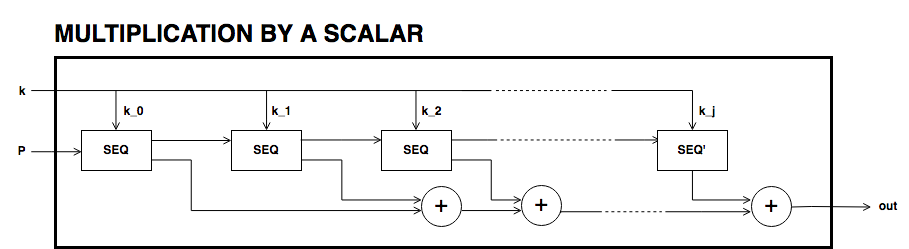
\includegraphics[scale=0.52]{figures/multiplication.png}
\end{figure}
\begin{multicols}{2}
%
\begin{enumerate}
\setcounter{enumi}{1}
	\item Each \textsc{seq} box takes a point of $E$ of the from $P_i = 2^{248 i} P$ for $i=0,\dots,j-1$ and outputs two points %of $E$,
	$$ 	2^{248} \cdot P_i 
		\quad \text{and} \quad
		\sum_{n = 0}^{247} b_n \cdot 2^{n} \cdot P_i. 
	$$
	The first point is the input of the next $(i+1)$-th \textsc{seq} box (note that $ 2^{248} \cdot P_i = P_{i+1}$) whereas the second output is the computation of the $i$-th term in expression (\ref{kP}). The precise circuit is depicted in next two figures \textsc{seq} and \textsc{window}.
	\vspace{-0.4cm}
	
	\item The idea of the circuit is to first compute %some point 		
			\begin{align*}
				Q =	& P_i + b_1 \cdot (2P_i) + b_2 \cdot (4P_i) \\
					&+ b_3 \cdot (8P_i) + \dots + b_{247} \cdot (2^{247}P_i),
			\end{align*}
	and output the point
		$$ Q - b_0 \cdot P_i. $$
	This permits the computation of $Q$ using the Montgomery form of Baby Jubjub and only use twisted Edwards for the second calculation. The reason to change forms is that, in the calculation of the output, we may get a sum with input the point at infinity if $b_0 = 0$. 
	
	Still, we have to ensure that none of the points being doubled or added when working in $E_M$ is the point at infinity and that we never add the same two points. 
	
	\begin{itemize}
		\item By assumption, $P\not= O$ and ord$(P)>8$. Hence, by Lagrange theorem {\cite[Corollary 4.12]{lagrange}}, $P$ must have order $r$, $2r$, $4r$ or $8r$. 
		For this reason, none of the points in $E_M$ being doubled or added in the circuit is the point at infinity, because for any integer $m$,  $2^m$ is never a multiple of $r$, even when $2^m$ is larger than $r$, as $r$ is a prime number. Hence, $2^m \cdot P \not= O$ for any $m\in\Z$.		
		
		\item Looking closely at the two inputs of the sum, it is easy to realize that they have different parity, one is an even multiple of $P_i$ and the other an odd multiple of $P_i$, so they must be different points. Hence, the sum in $E_M$ is done correctly.
	\end{itemize}
	
	\item The last term of expression (\ref{kP}) is computed in a very similar manner. The difference is that the number of bits composing $k_j$ may be shorter and that there is no need to compute $P_{j+1}$, as there is no other \textsc{seq} box after this one. So, there is only output, the point $k_j \cdot P_j = k_j\cdot 2^{248j} P$. This circuit is named \textsc{seq'}.

\end{enumerate}


\noindent The arithmetic on Baby Jubjub has already been implemented. Here are two available codes:
	\begin{itemize}
		\item Barry WhiteHat:
		\url{https://github.com/barryWhiteHat/baby_jubjub_ecc}
		\item iden3:
		\url{https://github.com/iden3/circomlib} 
	\end{itemize}

\end{multicols}
\begin{figure}[h]
	\centering
	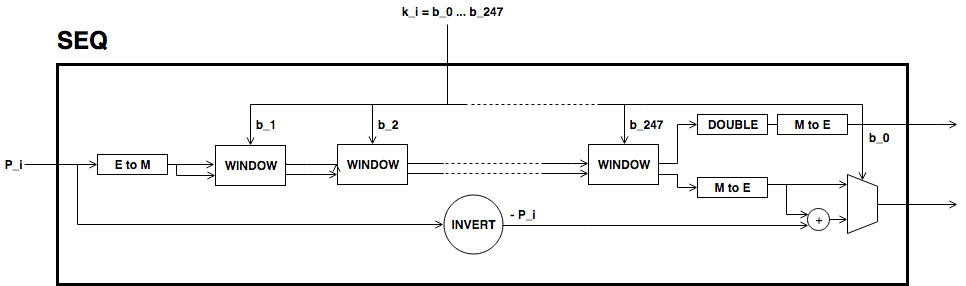
\includegraphics[scale=0.5]{figures/multiplication-SEQ.png}\\
	\vspace{1cm}
	
	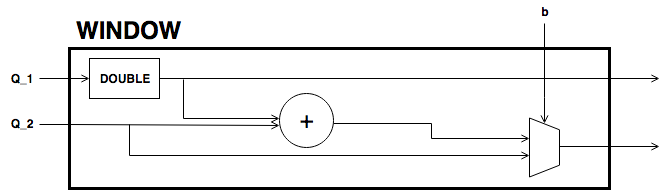
\includegraphics[scale=0.5]{figures/multiplication-SEQ-window.png}
	\vspace{0.3cm}
\end{figure}

\vspace{0.4cm}
\begin{multicols}{2}
\section {Intellectual Property}

To ensure it is freely available to everyone, we release this proposal under Creative Commons Attribution 4.0 International license. 
%See \url{https://creativecommons.org/licenses/by/4.0/} for a more detailed summary and the full text of the licence.

%%% References
\addcontentsline{toc}{section}{References}
	\bibliographystyle{acm}%{unsrt}
	\bibliography{lit}

\end{multicols}	

\newpage
\appendix

\section{Generation of Curves} \label{ap-gen}
\vspace{0.2cm}
\begin{lstlisting}
import sys
import pdb

def findCurve(prime, curveCofactor, twistCofactor, _A):
	F = GF(prime)
	A = _A
	while A < _A + 100000:
		print A
		if (A-2.) % 4 != 0:
			A+=1.
			continue
		try:
			E = EllipticCurve(F, [0, A, 0, 1, 0])
		except:
			A+=1.
			continue
		groupOrder = E.order()
		if (groupOrder % curveCofactor != 0
		or not is_prime(groupOrder // curveCofactor)):
			A+=1
			continue

		twistOrder = 2*(prime+1)-groupOrder
		if (twistOrder % twistCofactor != 0
		or not is_prime(twistOrder // twistCofactor)):
			A+=1
			continue
		return A, E

def find1Mod4(prime, curveCofactor, twistCofactor, A):
	assert((prime % 4) == 1)
	return findCurve(prime, curveCofactor, twistCofactor, A)
	
def find3Mod4(prime):
	assert((prime % 4) == 3)
	return findCurve(prime, 4, 4)

def findGenPoint(prime, A, EC, N):
	F = GF(prime)
	for uInt in range(1, 1e3):
		u = F(uInt)
		v2 = u^3 + A*u^2 + u
		if not v2.is_square():
			continue
		v = v2.sqrt()
	
		point = EC(u, v)
		pointOrder = point.order()
		if pointOrder == N:
			return point

def mont_to_ted(u, v , r):
	x = Mod(u / v, r) 
	y = Mod((u-1)/(u+1), r) 
	return(x, y)

def ted_to_mont(x, y , r):
	u = Mod((1 + y )/ ( 1 - y)  , r)
	v = Mod((1 + y ) / ( (1 - y) * x) , r ) 
	return(u,v)

def isOnEd(x,y,r,a,d):
	return Mod(Mod(a,r)*(x**2),r) + Mod(y**2 , r) - 1 
	- Mod(d,r)*(Mod(x**2,r))*(Mod(y**2,r)) == 0 
\end{lstlisting}
\vspace{0.4cm}

\section{Safety Criteria} \label{ap-safe}
\vspace{0.2cm}
\begin{lstlisting}
import os
import sys
from errno import ENOENT, EEXIST
from sortedcontainers import SortedSet


def readfile(fn):
  fd = open(fn,'r')
  r = fd.read()
  fd.close()
  return r

def writefile(fn,s):
  fd = open(fn,'w')
  fd.write(s)
  fd.close()

def expand2(n):
  s = ""
  
  while n != 0:
    j = 16
    while 2**j < abs(n): j += 1
    if 2**j - abs(n) > abs(n) - 2**(j-1): j -= 1
  
    if abs(abs(n) - 2**j) > 2**(j - 10):
      if n > 0:
        if s != "": s += " + "
        s += str(n)
      else:
        s += " - " + str(-n)
      n = 0
    elif n > 0:
      if s != "": s += " + "
      s += "2^" + str(j)
      n -= 2**j
    else:
      s += " - 2^" + str(j)
      n += 2**j
  
  return s

def requirement(fn,istrue):
  writefile(fn,str(istrue) + '\n')
  return istrue

def verify():
  try:
    os.mkdir('proof')
  except OSError as e:
    if e.errno != EEXIST: raise

  try:
    s = set(map(Integer, readfile('primes').split()))
  except IOError, e:
    if e.errno != ENOENT: raise
    s = set()

  needtofactor = SortedSet()
  V = SortedSet() # distinct verified primes
  verify_primes(V, s, needtofactor)
  verify_pass(V, needtofactor)

  old = V
  needtofactor.update(V)
  while len(needtofactor) > len(old):
    k = len(needtofactor) - len(old)
    sys.stdout.write('Factoring %d integer%s' % (k, '' if k == 1 else 's'))
    sys.stdout.flush()
    for x in needtofactor:
      if x not in old:
        for (y, z) in factor(x):
          s.add(y)
        sys.stdout.write('.')
        sys.stdout.flush()

    print('')

    old = needtofactor.copy()
    verify_primes(V, s, needtofactor)

  writefile('primes', '\n'.join(map(str, s)) + '\n')
  writefile('verify-primes', '<html><body>\n' +
                             ''.join(('2\n' if v == 2 else
                                      '<a href=proof/%s.html>%s</a>\n' % (v,v)) for v in V) +
                             '</body></html>\n')

  verify_pass(V, needtofactor)


def verify_primes(V, s, needtofactor):
  for n in sorted(s):
    if not n.is_prime() or n in V: continue
    needtofactor.add(n-1)
    if n == 2:
      V.add(n)
      continue
    for trybase in primes(2,10000):
      base = Integers(n)(trybase)
      if base^(n-1) != 1: continue
      proof = 'Primality proof for n = %s:\n' % n
      proof += '<p>Take b = %s.\n' % base
      proof += '<p>b^(n-1) mod n = 1.\n'
      f = factor(1)
      for v in reversed(V):
        if f.prod()^2 <= n:
          if n % v == 1:
            u = base^((n-1)/v)-1
            if u.is_unit():
              if v == 2:
                proof += '<p>2 is prime.\n'
              else:
                proof += '<p><a href=%s.html>%s is prime.</a>\n' % (v,v)
              proof += '<br>b^((n-1)/%s)-1 mod n = %s, which is a unit, inverse %s.\n' % (v,u,1/u)
              f *= factor(v)^(n-1).valuation(v)
      if f.prod()^2 <= n: continue
      if n % f.prod() != 1: continue
      proof += '<p>(%s) divides n-1.\n' % f
      proof += '<p>(%s)^2 > n.\n' % f
      proof += "<p>n is prime by Pocklington's theorem.\n"
      proof += '\n'
      writefile('proof/%s.html' % n,proof)
      V.add(n)
      break


def verify_pass(V, needtofactor):
  p = Integer(readfile('p'))
  k = GF(p)
  kz.<z> = k[]
  l = Integer(readfile('l'))
  x0 = Integer(readfile('x0'))
  y0 = Integer(readfile('y0'))
  x1 = Integer(readfile('x1'))
  y1 = Integer(readfile('y1'))
  shape = readfile('shape').strip()
  rigid = readfile('rigid').strip()

  safefield = True
  safeeq = True
  safebase = True
  saferho = True
  safetransfer = True
  safedisc = True
  saferigid = True
  safeladder = True
  safetwist = True
  safecomplete = True
  safeind = True

  pstatus = 'Unverified'
  if not p.is_prime(): pstatus = 'False'
  needtofactor.add(p)
  if p in V: pstatus = 'True'
  if pstatus != 'True': safefield = False
  writefile('verify-pisprime',pstatus + '\n')

  pstatus = 'Unverified'
  if not l.is_prime(): pstatus = 'False'
  needtofactor.add(l)
  if l in V: pstatus = 'True'
  if pstatus != 'True': safebase = False
  writefile('verify-lisprime',pstatus + '\n')

  writefile('expand2-p','= %s\n' % expand2(p))
  writefile('expand2-l','<br>= %s\n' % expand2(l))
  
  writefile('hex-p',hex(p) + '\n')
  writefile('hex-l',hex(l) + '\n')
  writefile('hex-x0',hex(x0) + '\n')
  writefile('hex-x1',hex(x1) + '\n')
  writefile('hex-y0',hex(y0) + '\n')
  writefile('hex-y1',hex(y1) + '\n')

  gcdlpis1 = gcd(l,p) == 1
  safetransfer &= requirement('verify-gcdlp1',gcdlpis1)

  writefile('verify-movsafe','Unverified\n')
  writefile('verify-embeddingdegree','Unverified\n')
  if gcdlpis1 and l.is_prime():
    u = Integers(l)(p)
    d = l-1
    needtofactor.add(d)
    for v in V:
      while d % v == 0: d /= v
    if d == 1:
      d = l-1
      for v in V:
        while d % v == 0:
          if u^(d/v) != 1: break
          d /= v
      safetransfer &= requirement('verify-movsafe',(l-1)/d <= 100)
      writefile('verify-embeddingdegree','<font size=1>%s</font><br>= (l-1)/%s\n' % (d,(l-1)/d))

  t = p+1-l*round((p+1)/l)
  if l^2 > 16*p:
    writefile('verify-trace','%s\n' % t)
    f = factor(1)
    d = (p+1-t)/l
    needtofactor.add(d)
    for v in V:
      while d % v == 0:
        d //= v
	f *= factor(v)
    writefile('verify-cofactor','%s\n' % f)
  else:
    writefile('verify-trace','Unverified\n')
    writefile('verify-cofactor','Unverified\n')

  D = t^2-4*p
  needtofactor.add(D)
  for v in V:
    while D % v^2 == 0: D /= v^2
  if prod([v for v in V if D % v == 0]) != -D:
    writefile('verify-disc','Unverified\n')
    writefile('verify-discisbig','Unverified\n')
    safedisc = False
  else:
    f = -prod([factor(v) for v in V if D % v == 0])
    if D % 4 != 1:
      D *= 4
      f = factor(4) * f
    Dbits = (log(-D)/log(2)).numerical_approx()
    writefile('verify-disc','<font size=1>%s</font><br>= <font size=1>%s</font><br>&#x2248; -2^%.1f\n' % (D,f,Dbits))
    safedisc &= requirement('verify-discisbig',D < -2^100)

  pi4 = 0.78539816339744830961566084581987572105
  rho = log(pi4*l)/log(4)
  writefile('verify-rho','%.1f\n' % rho)
  saferho &= requirement('verify-rhoabove100',rho.numerical_approx() >= 100)

  twistl = 'Unverified'
  d = p+1+t
  needtofactor.add(d)
  for v in V:
    while d % v == 0: d /= v
  if d == 1:
    d = p+1+t
    for v in V:
      if d % v == 0:
        if twistl == 'Unverified' or v > twistl: twistl = v

  writefile('verify-twistl','%s\n' % twistl)
  writefile('verify-twistembeddingdegree','Unverified\n')
  writefile('verify-twistmovsafe','Unverified\n')
  if twistl == 'Unverified':
    writefile('hex-twistl','Unverified\n')
    writefile('expand2-twistl','Unverified\n')
    writefile('verify-twistcofactor','Unverified\n')
    writefile('verify-gcdtwistlp1','Unverified\n')
    writefile('verify-twistrho','Unverified\n')
    safetwist = False
  else:
    writefile('hex-twistl',hex(twistl) + '\n')
    writefile('expand2-twistl','<br>= %s\n' % expand2(twistl))
    f = factor(1)
    d = (p+1+t)/twistl
    needtofactor.add(d)
    for v in V:
      while d % v == 0:
        d //= v
	f *= factor(v)
    writefile('verify-twistcofactor','%s\n' % f)
    gcdtwistlpis1 = gcd(twistl,p) == 1
    safetwist &= requirement('verify-gcdtwistlp1',gcdtwistlpis1)

    movsafe = 'Unverified'
    embeddingdegree = 'Unverified'
    if gcdtwistlpis1 and twistl.is_prime():
      u = Integers(twistl)(p)
      d = twistl-1
      needtofactor.add(d)
      for v in V:
        while d % v == 0: d /= v
      if d == 1:
        d = twistl-1
        for v in V:
          while d % v == 0:
            if u^(d/v) != 1: break
            d /= v
        safetwist &= requirement('verify-twistmovsafe',(twistl-1)/d <= 100)
        writefile('verify-twistembeddingdegree',"<font size=1>%s</font><br>= (l'-1)/%s\n" % (d,(twistl-1)/d))

    rho = log(pi4*twistl)/log(4)
    writefile('verify-twistrho','%.1f\n' % rho)
    safetwist &= requirement('verify-twistrhoabove100',rho.numerical_approx() >= 100)

    precomp = 0
    joint = l
    needtofactor.add(p+1-t)
    needtofactor.add(p+1+t)
    for v in V:
      d1 = p+1-t
      d2 = p+1+t
      while d1 % v == 0 or d2 % v == 0:
        if d1 % v == 0: d1 //= v
        if d2 % v == 0: d2 //= v
        # best case for attack: cyclic; each power is usable
	# also assume that kangaroo is as efficient as rho
        if v + sqrt(pi4*joint/v) < sqrt(pi4*joint):
	  precomp += v
	  joint /= v
        
    rho = log(precomp + sqrt(pi4 * joint))/log(2)
    writefile('verify-jointrho','%.1f\n' % rho)
    safetwist &= requirement('verify-jointrhoabove100',rho.numerical_approx() >= 100)


  x0 = k(x0)
  y0 = k(y0)
  x1 = k(x1)
  y1 = k(y1)

  if shape in ('edwards', 'tedwards'):
    d = Integer(readfile('d'))
    a = 1
    if shape == 'tedwards':
      a = Integer(readfile('a'))

    writefile('verify-shape','Twisted Edwards\n')
    writefile('verify-equation','%sx^2+y^2 = 1%+dx^2y^2\n' % (a, d))
    if a == 1:
      writefile('verify-shape','Edwards\n')
      writefile('verify-equation','x^2+y^2 = 1%+dx^2y^2\n' % d)

    a = k(a)
    d = k(d)
    elliptic = a*d*(a-d)
    level0 = a*x0^2+y0^2-1-d*x0^2*y0^2
    level1 = a*x1^2+y1^2-1-d*x1^2*y1^2

  if shape == 'montgomery':
    writefile('verify-shape','Montgomery\n')
    A = Integer(readfile('A'))
    B = Integer(readfile('B'))
    equation = '%sy^2 = x^3<wbr>%+dx^2+x' % (B,A)
    if B == 1:
      equation = 'y^2 = x^3<wbr>%+dx^2+x' % A
    writefile('verify-equation',equation + '\n')

    A = k(A)
    B = k(B)
    elliptic = B*(A^2-4)
    level0 = B*y0^2-x0^3-A*x0^2-x0
    level1 = B*y1^2-x1^3-A*x1^2-x1

  if shape == 'shortw':
    writefile('verify-shape','short Weierstrass\n')
    a = Integer(readfile('a'))
    b = Integer(readfile('b'))
    writefile('verify-equation','y^2 = x^3<wbr>%+dx<wbr>%+d\n' % (a,b))

    a = k(a)
    b = k(b)
    elliptic = 4*a^3+27*b^2
    level0 = y0^2-x0^3-a*x0-b
    level1 = y1^2-x1^3-a*x1-b

  writefile('verify-elliptic',str(elliptic) + '\n')
  safeeq &= requirement('verify-iselliptic',elliptic != 0)
  safebase &= requirement('verify-isoncurve0',level0 == 0)
  safebase &= requirement('verify-isoncurve1',level1 == 0)

  if shape in ('edwards', 'tedwards'):
    A = 2*(a+d)/(a-d)
    B = 4/(a-d)
    x0,y0 = (1+y0)/(1-y0),((1+y0)/(1-y0))/x0
    x1,y1 = (1+y1)/(1-y1),((1+y1)/(1-y1))/x1
    shape = 'montgomery'

  if shape == 'montgomery':
    a = (3-A^2)/(3*B^2)
    b = (2*A^3-9*A)/(27*B^3)
    x0,y0 = (x0+A/3)/B,y0/B
    x1,y1 = (x1+A/3)/B,y1/B
    shape = 'shortw'

  try:
    E = EllipticCurve([a,b])
    numorder2 = 0
    numorder4 = 0
    for P in E(0).division_points(4):
      if P != 0 and 2*P == 0:
        numorder2 += 1
      if 2*P != 0 and 4*P == 0:
        numorder4 += 1
    writefile('verify-numorder2',str(numorder2) + '\n')
    writefile('verify-numorder4',str(numorder4) + '\n')
    completesingle = False
    completemulti = False
    if numorder4 == 2 and numorder2 == 1:
      # complete edwards form, and montgomery with unique point of order 2
      completesingle = True
      completemulti = True
    # should extend this to allow complete twisted hessian
    safecomplete &= requirement('verify-completesingle',completesingle)
    safecomplete &= requirement('verify-completemulti',completemulti)
    safecomplete &= requirement('verify-ltimesbase1is0',l * E([x1,y1]) == 0)
    writefile('verify-ltimesbase1',str(l * E([x1,y1])) + '\n')
    writefile('verify-cofactorbase01',str(((p+1-t)//l) * E([x0,y0]) == E([x1,y1])) + '\n')
  except:
    writefile('verify-numorder2','Unverified\n')
    writefile('verify-numorder4','Unverified\n')
    writefile('verify-ltimesbase1','Unverified\n')
    writefile('verify-cofactorbase01','Unverified\n')
    safecomplete = False

  montladder = False
  for r,e in (z^3+a*z+b).roots():
    if (3*r^2+a).is_square():
      montladder = True
  safeladder &= requirement('verify-montladder',montladder)

  indistinguishability = False
  elligator2 = False
  if (p+1-t) % 2 == 0:
    if b != 0:
      indistinguishability = True
      elligator2 = True
  safeind &= requirement('verify-indistinguishability',indistinguishability)
  writefile('verify-ind-notes','Elligator 2: %s.\n' % ['No','Yes'][elligator2])

  saferigid &= (rigid == 'fully rigid' or rigid == 'somewhat rigid')

  safecurve = True
  safecurve &= requirement('verify-safefield',safefield)
  safecurve &= requirement('verify-safeeq',safeeq)
  safecurve &= requirement('verify-safebase',safebase)
  safecurve &= requirement('verify-saferho',saferho)
  safecurve &= requirement('verify-safetransfer',safetransfer)
  safecurve &= requirement('verify-safedisc',safedisc)
  safecurve &= requirement('verify-saferigid',saferigid)
  safecurve &= requirement('verify-safeladder',safeladder)
  safecurve &= requirement('verify-safetwist',safetwist)
  safecurve &= requirement('verify-safecomplete',safecomplete)
  safecurve &= requirement('verify-safeind',safeind)
  requirement('verify-safecurve',safecurve)

originaldir = os.open('.',os.O_RDONLY)
for i in range(1,len(sys.argv)):
  os.fchdir(originaldir)
  os.chdir(sys.argv[i])
verify()
\end{lstlisting}
\vspace{0.4cm}

\section{Generation of Baby Jubjub} \label{ap-baby}
\vspace{0.2cm}
\begin{lstlisting}
prime = 21888242871839275222246405745257275088548364400416034343698204186575808495617
Fr = GF(prime)
h = 8 # cofactor

A = int(sys.argv[1])
A, EC = find1Mod4(prime, h, 4, A)

B = 1
a = Fr((A + 2) / B)
d = Fr((A - 2) / B)

print "a " , a , "d " , d , sqrt(d)
# check we have a safe twist
assert(not d.is_square())
assert(a*d*(a-d)!=0)

s = factor(EC.order())
print ("l : " , s)
N = h * s # order of the curve
print (factor(EC.quadratic_twist().order()))

# get generator point
u_gen, v_gen, w_gen = findGenPoint(prime, A, EC, N)
# find that generator point on the edwards curve
gen_x, gen_y = mont_to_ted(u_gen, v_gen, prime)
# make sure the generator point is on the twisted edwards curve
assert(isOnEd(gen_x, gen_y, prime, a , d))
# go back to montgomery
u , v = ted_to_mont(gen_x, gen_y, prime)
# confirm we are back where we started from
assert (u == u_gen)
assert (v == v_gen)

# get base point on montgomery curve by multiplying the generator point by h
base_x , base_y, base_z = h*EC(u_gen, v_gen)
# find the same points on twisted edwards curve
base_x , base_y = mont_to_ted(base_x , base_y, prime)

# the generator is on the twisted edwards curve
assert(isOnEd(base_x,base_y, prime , a , d))

print ("generator :" , gen_x, gen_y)
print ("base :", base_x, base_y)
\end{lstlisting}

\end{spacing}	
\end{document}
